\documentclass[xetex,hyperref={pdfpagelabels=false}]{beamer}

% --------------------------------------------------------------------------
% Color definitions.
% --------------------------------------------------------------------------
\usepackage{xcolor}
\definecolor{aliceblue}{rgb}{0.94, 0.97, 1.0}
\definecolor{amber}{rgb}{1.0, 0.75, 0.0}
\definecolor{amethyst}{rgb}{0.6, 0.4, 0.8}
\definecolor{antiquefuchsia}{rgb}{0.57, 0.36, 0.51}
\definecolor{ashgrey}{rgb}{0.7, 0.75, 0.71}
\definecolor{ballblue}{rgb}{0.13, 0.67, 0.8}
\definecolor{blue(munsell)}{rgb}{0.0, 0.5, 0.69}
\definecolor{blue(pigment)}{rgb}{0.2, 0.2, 0.6}
\definecolor{blu}{RGB}{1,0,102}
\definecolor{bondiblue}{rgb}{0.0, 0.58, 0.71}
\definecolor{brightmaroon}{rgb}{0.76, 0.13, 0.28}
\definecolor{cadet}{rgb}{0.33, 0.41, 0.47}


% --------------------------------------------------------------------------
% My palette.
% --------------------------------------------------------------------------
\definecolor{energy}{RGB}{49,247,250}
\definecolor{delicate}{RGB}{67,179,223}
\definecolor{faded}{RGB}{76,117,195}
\definecolor{plum}{RGB}{87,78,164}
\definecolor{petunias}{RGB}{109,80,139}
\definecolor{letour}{RGB}{101,41,105}

% --------------------------------------------------------------------------

% --------------------------------------------------------------------------
% Beamer configuration.
% --------------------------------------------------------------------------
\usetheme{default}
\usecolortheme{default}
\usefonttheme{serif}

\beamertemplatenavigationsymbolsempty
\setbeamertemplate{navigation symbols}{}
\hypersetup{pdfpagemode=UseNone}

% footer.
\setbeamercolor{headFoot}{fg=white, bg=plum!80!black}
\setbeamertemplate{footline}{
  \leavevmode%
  \hbox{%
  \begin{beamercolorbox}
    [wd=.8\paperwidth,ht=2.3ex,dp=1ex,left]{headFoot}%
    \hspace*{2ex}\insertshorttitle\hspace*{2mm}(\insertshortauthor)
  \end{beamercolorbox}%
  \begin{beamercolorbox}
    [wd=.2\paperwidth,ht=2.3ex,dp=1ex,right]{headFoot}%
    \insertframenumber{}/\inserttotalframenumber\hspace*{2ex}
  \end{beamercolorbox}}%
  \vskip0pt%
}

% title in the frame
\setbeamerfont{frametitle}{size=\small,series=\bfseries}
\setbeamercolor{frametitle}{fg=white,bg=plum}

\setbeamerfont{framesubtitle}{size=\normalfont\tiny\itshape}
\setbeamercolor{framesubtitle}{fg=white, bg=plum}

\setbeamercolor{background canvas}{bg=white}
\setbeamercolor{normal text}{fg=black}

% \setbeamercolor{institute}{fg=blu}
% \setbeamercolor{subtitle}{fg=blu}
% \setbeamercolor{titlelike}{fg=blu}
\setbeamerfont{footnote}{size=\tiny}
\setbeamercolor{footnote}{fg=gray}
% \setbeamercolor{block title}{bg=blue,fg=blu}
% \setbeamercolor{block body}{bg=aliceblue}
% \setbeamercolor{item}{fg=blu} % color of bullets
% \setbeamercolor{subitem}{fg=blu}
% \setbeamercolor{itemize/enumerate subbody}{fg=blu}
% \setbeamertemplate{itemize subitem}{{\textendash}}
% \setbeamerfont{itemize/enumerate subbody}{size=\footnotesize}
% \setbeamerfont{itemize/enumerate subitem}{size=\footnotesize}

% --------------------------------------------------------------------------

\usepackage[english]{babel}
\usepackage{amsmath, amsthm, amssymb}
\usepackage{bussproofs}
\usepackage{fancyvrb}
\usepackage{geometry}
\usepackage{graphicx}
\usepackage{lmodern}
\usepackage{lstagda}
\usepackage{tikz}
\usepackage{url}

\usefonttheme{professionalfonts}
\usefonttheme{serif}
\usepackage{fontspec}
\usepackage{mathtools}
\usepackage{unicode-math}

\setmathfont[ExternalLocation=fonts/
  , BoldFont=xits-mathbold.otf
  ]{xits-math.otf}

\setmainfont[ExternalLocation=fonts/
  , BoldFont=SourceSansPro-Semibold.otf
  , BoldItalicFont=SourceSansPro-SemiboldIt.otf
  , ItalicFont=SourceSansPro-It.otf
  ]{SourceSansPro-Regular.otf}

\setmonofont[ExternalLocation=fonts/
  , BoldFont=SourceCodePro-Semibold.ttf
  , BoldItalicFont=SourceCodePro-SemiboldIt.ttf
  , ItalicFont=SourceCodePro-It.ttf
  ]{SourceCodePro-Semibold.ttf}
\newfontfamily\SourceCodeIt{fonts/SourceCodePro-It.ttf}
\newfontfamily\SourceCode{fonts/SourceCodePro-Regular.ttf}

\newcommand{\problemtptp}[3][c]
  {\lstinputlisting[style=tptp,caption=#2, firstline=#3, label=custom#1]{#2}}
\newcommand{\solutiontstp}[2][c]
  {\lstinputlisting[style=tptp,caption=#2, firstline=5, label=custom#1]{#2}}

% --------------------------------------------------------------------------
% References
\usepackage[autostyle]{csquotes}
\usepackage[
    backend=biber
  , style=authoryear-icomp
  , sortlocale=en_US
  , natbib=true
  , url=false
  , doi=true
  , eprint=false
]{biblatex}
\addbibresource{ref.bib}
\renewcommand*{\nameyeardelim}{\addcomma\addspace}
\usepackage{silence}
\WarningFilter{biblatex}{Patching footnotes failed}

% --------------------------------------------------------------------------
% Title Page
\title{\textbf{Proof Reconstruction in Classical Propositional Logic}}
\date{Agda Implementors’ Meeting XXV\\
May 9-15th}
\author{Jonathan Prieto-Cubides}

\institute{
Advisor: Andr\'es Sicard-Ram\'irez\\[3mm]
Universidad EAFIT\\
Medell\'in, Colombia}
% --------------------------------------------------------------------------

\newsavebox\agdapragma

\begin{document}


\setcounter{page}{1}

\begin{frame}[plain]
% \tikz[overlay,remember picture] \node[opacity=0.05, at=(6,6)] {
% $Γ ⊢ ϕ$
% };
\titlepage
\end{frame}


\begin{frame}
  \frametitle{Outline}
  \tableofcontents
\end{frame}

\section{Introduction}
\subsection{Motivation}


\begin{lrbox}{\agdapragma}
\begin{lstlisting}
$ cat Or.agda
module Or where

data _or_ (A B : Set) : Set where
  inj1 : A -> A or B
  inj2 : B -> A or B

postulate
  A B    : Set
  or-comm : A or B -> B or A
{-# ATP prove or-comm #-}
\end{lstlisting}
\end{lrbox}

\begin{frame}[fragile]{Translation}

\only<1-2>{At the moment, the communication between Agda and
the ATPs is unidirectional because the ATPs are being used as oracles.\citep{Sicard2015}.}
\only<1-2>{\vfill}

\begin{tikzpicture}[scale=2]
\only<1->{ \node(agda-pragmas) at (0,0){
\includegraphics{figures/agda-pragmas.pdf}}};
\only<1>{
  \node[fill=aliceblue, rectangle](atp-pragma) at (3,0){
  \scalebox{0.7}{\usebox\agdapragma}
  }};


\only<2->{ \node(eagda) at (2,0){
  
\includegraphics{figures/eagda.pdf}
  \footnote{Development version of Agda in order to handle a new built-in ATP-pragma.
    \url{https://github.com/asr/eagda}}
  }};

\only<3->{ \node(apia) at (4,0){
  
\includegraphics{figures/apia.pdf}
  \footnote{Haskell program for proving first-order theorems written in Agda using ATPs.
    \url{https://github.com/asr/apia}}}
  };

\only<3->{ \node(tptp) at (2,-2){
\includegraphics{figures/tptp.pdf}}};

\only<3->{ \node(atp) at (4,-2){
\includegraphics{figures/atp.pdf}}};

\only<2->{\draw[->,ultra thick] (agda-pragmas) to (eagda)};

\only<3->{\draw[->,ultra thick] (eagda) to (apia)};
\only<3->{\draw[->, very thick, dashed, gray] (apia) to (tptp)};
\only<3->{\draw[->, very thick, dashed, gray] (tptp) to (atp)};
\only<3->{\draw[->, very thick, dashed, gray] (atp) to (apia)};

\end{tikzpicture}

\end{frame}

% \subsection{Proof Reconstruction}

% \subsubsection{Sledgehammer}
% \subsubsection{Waldemesiter}

\subsection{Automatic Provers}

\subsubsection{TPTP Syntax}

\begin{frame}[fragile]{TPTP Syntax}{Thousands of Problems for Theorem Provers}
\label{tptp-syntax}
 \tikz[overlay,remember picture]
  \node at (0.92\textwidth, 0cm)
    {
\includegraphics[width=0.15\textwidth]{figures/tptp}};

  \begin{itemize}
  \item Is a language\footnote{Is available at
        \url{http://www.cs.miami.edu/~tptp/TPTP/SyntaxBNF.html}}
        to encode problems in text files
  \item Is the input of the ATPs
  \item his problems contains formulas with the form
   \begin{center}
\begin{verbatim}
language(name, role, formula).
\end{verbatim}
    \end{center}
    \begin{itemize}
      \item[\texttt{language}] THF, TFF, FOF, or CNF
      \item[\texttt{name}] to identify the formula within the problem
      \item[\texttt{role}] axiom, definition, hypothesis, conjecture, among others
      \item[\texttt{formula}] the logic formula in the language
    \end{itemize}
  \end{itemize}
\end{frame}

\begin{frame}[fragile]{TPTP Examples}{Prop-Pack Repository}
\label{tptp-examples}
Problems in Propositional Logic:
  \begin{itemize}
    \item $p ⊢ p$
\begin{tptp}
$ cat basic-4.tptp
fof(a, axiom, p).
fof(goal, conjecture, p).
\end{tptp}
    \item $p ∧ q ⊢ q ∧ p$
\begin{tptp}
$ cat conj-3.tptp
fof(a, axiom, p & q).
fof(goal, conjecture, q & p).
\end{tptp}
    \item $⊢ ¬ (p ∧ ¬ p) ∨ (q ∧ ¬ q)$
\begin{tptp}
$ cat neg-7.tptp
fof(goal, conjecture, ~ ((p & ~ p) | (q & ~ q))).
\end{tptp}
    \end{itemize}
\end{frame}

\subsubsection{TSTP Derivations}

\begin{frame}[fragile]{TSTP Syntax}
\label{tstp-syntax}
 \tikz[overlay,remember picture]
  \node at (0.92\textwidth, -0.5cm)
    {
\includegraphics[width=0.15\textwidth]{figures/tstp}};


A TSTP derivation
\footnote{\url{http://www.cs.miami.edu/~tptp/TPTP/QuickGuide/Derivations.html}}
\begin{itemize}
  \item Is a Directed Acyclic Graph where
  \begin{itemize}
    \item[\texttt{leaf}] is a formulae from the TPTP input
    \item[\texttt{node}] is a formulae inferred from parent formulae
    \item[\texttt{root}] the final derived formulae
  \end{itemize}
  \item Is a list of annotated formulae:
  {\footnotesize
    \begin{center}
\begin{verbatim}
language(name,role,formula,source[,useful info]).
\end{verbatim}
  \end{center}}
\begin{itemize}
  \item[\texttt{source}] typically is a inference record:
    {\footnotesize
\begin{verbatim}
  inference(rule, [], [])
  \end{verbatim}}
\begin{itemize}
    \item[-] The inference rule name,
    \item[-] a list of useful inference information, and
    \item[-] a list of references to its parent formulae.
\end{itemize}
\end{itemize}
\end{itemize}
\end{frame}

\begin{frame}[fragile]{TSTP Example}
\label{tstp-example}
 \tikz[overlay,remember picture]
  \node at (0.93\textwidth, -0.3cm)
    {
\includegraphics[width=0.15\textwidth]{figures/metis}};

\begin{itemize}
  \item Proof found by \texttt{Metis} ATP for the problem $p ⊢ p$
\begin{tptp}
$ metis --show proof basic-4.tptp
fof(a, axiom, (p)).
fof(goal, conjecture, (p)).
fof(subgoal_0, plain, (p),
  inference(strip, [], [goal])).
fof(negate_0_0, plain, (~ p),
  inference(negate, [], [subgoal_0])).
fof(normalize_0_0, plain, (~ p),
  inference(canonicalize, [], [negate_0_0])).
fof(normalize_0_1, plain, (p),
  inference(canonicalize, [], [a])).
fof(normalize_0_2, plain, ($false),
  inference(simplify, [],
    [normalize_0_0, normalize_0_1])).
cnf(refute_0_0, plain, ($false),
    inference(canonicalize, [], [normalize_0_2])).
\end{tptp}
\end{itemize}
\end{frame}


\begin{frame}[fragile]{DAG for the previous TSTP derivation found by \texttt{Metis} ATP}
\label{tstp-dag}
\vfill
\begin{center}
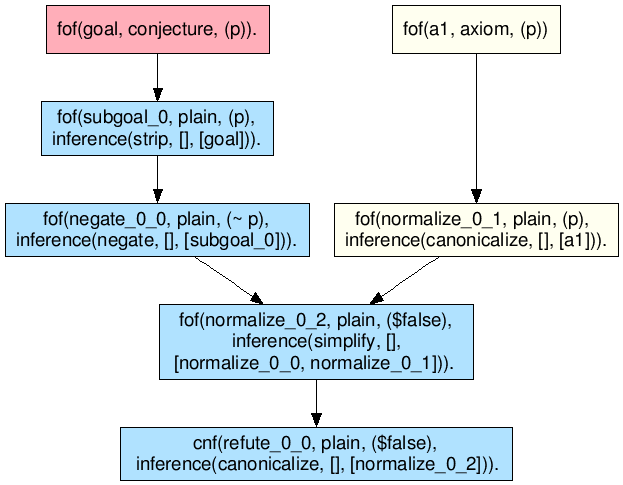
\includegraphics[height=0.8\textheight]{figures/derivation.png}
\end{center}
\end{frame}

\begin{frame}{Design decisions for the Reconstruction Tool}
\label{agda}

 \tikz[overlay,remember picture]
  \node at (0.93\textwidth, 0cm)
    {
\includegraphics[width=0.2\textwidth]{figures/athena}};

\textbf{Programming Languages}
\begin{itemize}
\item \texttt{Haskell} is a standardized, general-purpose purely functional programming language.\\
Our usages:
\begin{itemize}
    \item Parsing
    \item AST construction
    \item Creation and analysis of DAG derivations
    \item Analysis of inference rules used
    \item Generation of Agda code of the proof
\end{itemize}

\item \texttt{Agda} is dependently typed functional programming language and it also a proof assistant.\\
Our usages:
    \begin{itemize}
    \item Logic framework for Classical Propositional Logic
    \item Type-Checker for the Agda code of the proofs generated
    \end{itemize}
\end{itemize}






\end{frame}


\begin{frame}{References}
\label{references}
\printbibliography
\end{frame}

\end{document}